\documentclass[10pt, letterpaper]{article}
\usepackage[cm]{fullpage}
\usepackage{algpseudocode}
\usepackage{algorithm}
\usepackage{graphicx}
\usepackage[section]{placeins}
\usepackage[table]{xcolor}
\usepackage{amsmath}
\usepackage[margin=0.7in]{geometry}
\usepackage{comment}
\usepackage{wrapfig}

\algrenewcommand\Return{\State \algorithmicreturn{} }%

\title{Tetanus - A Batch GCD RSA Cracker}
\author{Daiwei Chen \and Cole Houston}
\date{\today}

\begin{document}
\maketitle
\begin{abstract}

\end{abstract}

\section{Background and Related Work}


\section{RSA}
Let's quickly go over RSA, how it is possible to break it. RSA is usually cryptographically secure due to the complexity and difficulty to factor very, very large prime numbers. However, within the Public Component of RSA contains $N$, a result of the product between two (usually) large primes $p$ and $q$. However, if one could efficiently calcualte $p$ and $q$ from $N$, then it will be possible to reconstruct a RSA Private key. \\
\\
This means it is possible to perform Man In the Middle attacks against the cracked RSA Private Key target. Decrypt TLS encrypted traffic, or even authenticate SSH using the public key as well. Essentially, you become your target.

\section{Batch GCD}
\begin{wrapfigure}{r}{0.5\textwidth}
  \begin{center}
    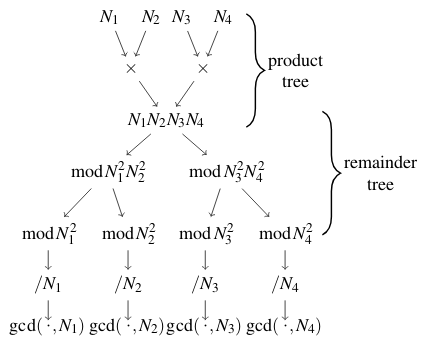
\includegraphics[width=0.48\textwidth]{batch-gcd-tree.png}
  \end{center}
  \caption{The Batch GCD Trees and how they're created and used.}
\end{wrapfigure}

Batch GCD is split into 3 main components: creation of the product tree, creation of the remainder tree, and finally, the GCD process.

\begin{enumerate}
\item Creation of the product tree. \\
  The base of the product tree is simply the RSA moduli. The product tree is created by multiplying 2 numbers to create a new layer, and keep multiplying every next 2 numbers together till you run out of numbers. On odd layers, simply add the final number to the end. Stop creating more layers until you reach the final number.
\item Creation of the remainder tree. \\
  The remainder tree is created by first using the final number of the product tree. Then, for each new layer, the $i/2$th product number in that layer is modded to with then $i$th number on the next layer of the product tree squared. This is a faster version of Batch-GCD, in the slower version, you simply create the final layer of the remainder tree by modding the final product tree number to each moduli.
\item Performing the GCD. \\
  Finally, for each moduli, find the GCD between each number on the final layer of the remainder tree divide by the modulus and the modulus itself.
\end{enumerate}

\section{Experimental Setup}
We have collected about 22,000 keys all together from 2 main sources for this project. First, we grabbed a datadump of about 10,000 moduli from 
\section{Results}

\section{Conclusions}

\end{document}
